%% 
%% Copyright 2007, 2008, 2009 Elsevier Ltd
%% 
%% This file is part of the 'Elsarticle Bundle'.
%% ---------------------------------------------
%% 
%% It may be distributed under the conditions of the LaTeX Project Public
%% License, either version 1.2 of this license or (at your option) any
%% later version.  The latest version of this license is in
%%    http://www.latex-project.org/lppl.txt
%% and version 1.2 or later is part of all distributions of LaTeX
%% version 1999/12/01 or later.
%% 
%% The list of all files belonging to the 'Elsarticle Bundle' is
%% given in the file `manifest.txt'.
%% 
%% Template article for Elsevier's document class `elsarticle'
%% with harvard style bibliographic references
%% SP 2008/03/01

%\documentclass[preprint,12pt,authoryear]{elsarticle}  %default in the template
%\documentclass[preprint,10pt,authoryear]{elsarticle}

%% Use the option review to obtain double line spacing
%% \documentclass[authoryear,preprint,review,12pt]{elsarticle}

%% Use the options 1p,twocolumn; 3p; 3p,twocolumn; 5p; or 5p,twocolumn
%% for a journal layout:
%% \documentclass[final,1p,times,authoryear]{elsarticle}
%% \documentclass[final,1p,times,twocolumn,authoryear]{elsarticle}
 \documentclass[final,3p,times,authoryear]{elsarticle}
%% \documentclass[final,3p,times,twocolumn,authoryear]{elsarticle}
%% \documentclass[final,5p,times,authoryear]{elsarticle}
%% \documentclass[final,5p,times,twocolumn,authoryear]{elsarticle}

%% For including figures, graphicx.sty has been loaded in
%% elsarticle.cls. If you prefer to use the old commands
%% please give \usepackage{epsfig}

%% The amssymb package provides various useful mathematical symbols
\usepackage{amssymb}
%% The amsthm package provides extended theorem environments
 \usepackage{amsthm}
 \usepackage{amsmath}
 \usepackage{color}
 \usepackage{amsmath}
\usepackage{siunitx}


\usepackage{framed} % Framing content
\usepackage{multicol} % Multiple columns environment
\usepackage{nomencl} % Nomenclature package
\makenomenclature
%\setlength{\nomitemsep}{-\parskip} % Baseline skip between items
\setlength{\nomitemsep}{0.01cm}
\renewcommand*\nompreamble{\begin{multicols}{2}}
\renewcommand*\nompostamble{\end{multicols}}
\newcommand{\degreeC}{\ensuremath{^\circ}C }

\usepackage[nonumberlist]{glossaries}
\makeglossaries 


%% The lineno packages adds line numbers. Start line numbering with
%% \begin{linenumbers}, end it with \end{linenumbers}. Or switch it on
%% for the whole article with \linenumbers.
%% \usepackage{lineno}

\journal{Urban Climate}

\newglossaryentry{Tsurf}{name={$T_{surf}$},symbol={\ensuremath{T_{surf}}},description={surface temperature from the force-restore model (\degreeC)}}
\newglossaryentry{Toolkit2}{name={Toolkit-2},symbol={Toolkit-2},description={CRC for Water Sensitive Cities micro-climate toolit model}}
\newglossaryentry{Tac}{name={$T_{ac}$},symbol={\ensuremath{T_{ac}}},description={street level (urban canopy layer) air temperature (\degreeC)}}
\newglossaryentry{Uz}{name={$U_{z}$},symbol={\ensuremath{U_{z}}},description={BoM reference wind speed (m s$^{-1}$)}}
\newglossaryentry{Tb}{name={$T_{b}$},symbol={\ensuremath{T_{b}}},description={the air temperature above the urban canopy layer (\degreeC)}}
\newglossaryentry{Fbldg}{name={$F_{bldg}$},symbol={$F_{bldg}$},description={land cover building fraction (\%)}} 
\newglossaryentry{Fconc}{name={$F_{conc}$},symbol={$F_{conc}$},description={land cover concrete fraction (\%)}} 
\newglossaryentry{Fasph}{name={$F_{asph}$},symbol={$F_{asph}$},description={land cover asphalt fraction (\%)}} 
\newglossaryentry{Fgras}{name={$F_{gras}$},symbol={$F_{gras}$},description={land cover grass fraction (\%)}} 
\newglossaryentry{Figrs}{name={$F_{igrs}$},symbol={$F_{igrs}$},description={land cover irrigated grass fraction (\%)}} 
\newglossaryentry{Ftree}{name={$F_{tree}$},symbol={$F_{tree}$},description={land cover tree fraction (\%)}} 
\newglossaryentry{Fwatr}{name={$F_{watr}$},symbol={$F_{watr}$},description={land cover water fraction (\%)}} 
\newglossaryentry{W}{name={$W$},symbol={\ensuremath{W}},description={average street width (m)}}
\newglossaryentry{BH}{name={$hH_{b}$},symbol={\ensuremath{h_{b}}},description={average building height (m)}}
\newglossaryentry{kdown}{name={$K\downarrow$},symbol={\ensuremath{K\downarrow}},description={incoming shortwave radiation (W m$^{-2}$)}}
\newglossaryentry{lup}{name={$L\uparrow$},symbol={\ensuremath{L\uparrow}},description={outgoing longwave radiation (W m$^{-2}$)}}
\newglossaryentry{ldown}{name={$L\downarrow$},symbol={\ensuremath{L\downarrow}},description={incoming longwave radiation (W m$^{-2}$)}}
\newglossaryentry{l*}{name={$L_{n}$},symbol={\ensuremath{L_{n}}},description={net longwave radiation (W m$^{-2}$)}}
\newglossaryentry{k*}{name={$K_{n}$},symbol={\ensuremath{K_{n}}},description={net shortwave radiation (W m$^{-2}$)}}
\newglossaryentry{RH}{name={$RH$},symbol={\ensuremath{RN}},description={relative humidity (\%)}}
\newglossaryentry{Ta}{name={$T_{a}$},symbol={\ensuremath{T_{a}}},description={air temperature from the nearest BoM site (2 m) (\degreeC)}}
\newglossaryentry{Rn}{name={$R_{n}$},symbol={\ensuremath{R_{n}}},description={net radiation (W m$^{-2}$)}}
\newglossaryentry{albedo}{name={$\alpha$},symbol={\ensuremath{\alpha}},description={surface albedo}}
\newglossaryentry{epsilon}{name={$\epsilon$},symbol={\ensuremath{\epsilon}},description={surface emissivity}}
\newglossaryentry{sigma}{name={$\sigma$},symbol={\ensuremath{\sigma}},description={Stefan-Boltzmann constant (=5.67 $\times$ 10$^{-8}$ W m$^{-2}$K$^{-4}$)}} 
\newglossaryentry{H}{name={$H$},symbol={\ensuremath{H}},description={sensible heat flux from LUMPS (W m$^{-2}$)}}
\newglossaryentry{LE}{name={$LE$},symbol={\ensuremath{LE}},description={latent heat flux from LUMPS (W m$^{-2}$)}}
\newglossaryentry{pm}{name={$pm$},symbol={\ensuremath{pm}},description={LUMPS empirical parameter (`alpha’ parameter) - relates to surface moisture}}
\newglossaryentry{s}{name={$s$},symbol={\ensuremath{s}},description={slope of the saturation vapour pressure-versus-temperature curve }} 
\newglossaryentry{gamma}{name={$\gamma$},symbol={\ensuremath{\gamma}},description={psychrometric constant}}
\newglossaryentry{DeltaS}{name={$\Delta S$},symbol={\ensuremath{\Delta S}},description={storage heat flux from LUMPS (W m$^{-2}$)}}
\newglossaryentry{beta}{name={$\beta$},symbol={\ensuremath{\beta}},description={LUMPS empirical parameter (beta parameter)}}
\newglossaryentry{betak}{name={$\beta_{k}$},symbol={\ensuremath{\beta_{k}}},description={amount of shortwave radiation immediately absorbed by the water layer (set to 0.45)}}
\newglossaryentry{a1}{name={$a_{1}$},symbol={\ensuremath{a_{1}}},description={Objective hysteresis model (OHM) parameter}}
\newglossaryentry{a2}{name={$a_{2}$},symbol={\ensuremath{a_{2}}},description={Objective hysteresis model (OHM) parameter}}
\newglossaryentry{a3}{name={$a_{3}$},symbol={\ensuremath{a_{3}}},description={Objective hysteresis model (OHM) parameter}}
\newglossaryentry{C}{name={$C$},symbol={\ensuremath{C}},description={volumetric heat capacity (J m$^{-3}$ K$^{-1}$)}}
\newglossaryentry{kappa}{name={$\kappa$},symbol={\ensuremath{\kappa}},description={thermal diffusivity (m$^{2}$ s$^{-1}$)}}
\newglossaryentry{Tm}{name={$T_{m}$},symbol={\ensuremath{T_{m}}},description={average soil (ground) temperature (\degreeC)}}
\newglossaryentry{Dy}{name={$D_{y}$},symbol={\ensuremath{D_{y}}},description={damping depth for the annual temperature cycle (m)}}
\newglossaryentry{Sab}{name={$S_{ab}$},symbol={\ensuremath{S_{ab}}},description={absorbed shortwave radiation (W m$^{-2}$)}}
\newglossaryentry{Gwtr}{name={$G_{wtr}$},symbol={\ensuremath{G_{wtr}}},description={convective heat flux at the bottom of the water layer (and into the soil below) (W m$^{-2}$)}}
\newglossaryentry{deltaSwtr}{name={$\Delta S_{wtr}$},symbol={\ensuremath{\Delta S_{wtr}}},description={change in heat storage of the water layer (W m$^{-2}$)}}
\newglossaryentry{eta}{name={$\eta$},symbol={\ensuremath{\eta}},description={extinction coefficient}}
\newglossaryentry{Cwtr}{name={$C_{wrt}$},symbol={\ensuremath{C_{wrt}}},description={volumetric heat capacity of water (4.18$\times$10$^{6}$ J m$^{-3}$ K$^{-1}$)}}
\newglossaryentry{kwtr}{name={$\kappa_{wtr}$},symbol={\ensuremath{\kappa_{wtr}}},description={eddy diffusivity of water (m$^{2}$ s$^{-1}$)}}
\newglossaryentry{Twtr}{name={$T_{wtr}$},symbol={\ensuremath{T_{wtr}}},description={water surface temperature from simple water-body model (\degreeC)}}
\newglossaryentry{Ts}{name={$T_{s}$},symbol={\ensuremath{T_{s}}},description={soil temperature (\degreeC)}}
\newglossaryentry{rhov}{name={$\rho v$},symbol={\ensuremath{\rho v}},description={density of moist air (kg m$^{-3}$)}}
\newglossaryentry{Lv}{name={$L_{v}$},symbol={\ensuremath{L_{v}}},description={latent heat of vaporisation (=2.43 MJ kg$^{-1}$)}}
\newglossaryentry{hv}{name={$h_{v}$},symbol={\ensuremath{h_{v}}},description={bulk transfer coefficient for moisture (=1.4 $\times$ 10$^{-3}$)}}  
\newglossaryentry{qa}{name={$q_{a}$},symbol={\ensuremath{q_{a}}},description={specific humidity (kg kg$^{-1}$)}}
\newglossaryentry{qs}{name={$q_{s}$},symbol={\ensuremath{q_{s}}},description={saturated specific humidity (kg kg$^{-1}$) }}  
\newglossaryentry{rhoa}{name={$\rho_{a}$},symbol={\ensuremath{\rho_{a}}},description={density of dry air (=1.2 kg m$^{-3}$)}} 
\newglossaryentry{cp}{name={$c_{p}$},symbol={\ensuremath{c_{p}}},description={specific heat of air (1013 J kg$^{-1}$ K$^{-1}$)}}
\newglossaryentry{hc}{name={$h_{c}$},symbol={\ensuremath{h_{c}}},description={bulk transfer coefficient for heat ($h_{c} = h_{v}$)}}
%\newglossaryentry{Cwtr}{name={$C_{wtr}$},symbol={\ensuremath{C_{wtr}}},description={volumetric heat capacity of water (J m$^{-2}$ K$^{-1}$)}}
\newglossaryentry{ra}{name={$r_{a}$},symbol={\ensuremath{r_{a}}},description={resistance from urban canopy to the atmosphere (s m$^{-1}$)}}
\newglossaryentry{zu}{name={$z_{u}$},symbol={\ensuremath{z_{u}}},description={BoM wind speed measurement height (typically 10 m)}}
\newglossaryentry{d}{name={$d$},symbol={\ensuremath{d}},description={zero plane displacement height (2/3 height of roughness elements, m)}}  
\newglossaryentry{z0}{name={$z_{0}$},symbol={\ensuremath{z_{0}}},description={roughness length (0.1 $\times$ height of roughness elements)}}  

\newglossaryentry{Hca}{name={$H_{ca}$},symbol={\ensuremath{H_{ca}}},description={conductance from urban canopy to the atmosphere (m s$^{-1}$)}}
\newglossaryentry{Hcs}{name={$H_{cs}$},symbol={\ensuremath{H_{cs}}},description={conductance from surface to canopy (m s$^{-1}$)}}
\newglossaryentry{rs}{name={$r_{s}$},symbol={\ensuremath{r_{s}}},description={resistance from surface to canopy (s m$^{-1}$)}}
\newglossaryentry{Ucan}{name={$U_{can}$},symbol={\ensuremath{U_{can}}},description={wind speed in canyon (m s$^{-1}$)}}
\newglossaryentry{Utop}{name={$U_{top}$},symbol={\ensuremath{U_{top}}},description={wind speed at the top of the canyon (m s$^{-1}$)}}
  
\newglossaryentry{aa}{name={$a$},symbol={\ensuremath{a}},description={a}}

 
%hv = bulk transfer coefficient for moisture (1.4×10$^{-3}$) 

%ra = resistance from urban canopy to the atmosphere (s m$^{-1}$)	


%βK = amount of shortwave radiation immediately absorbed by the water layer (set to 0.45)
%η = extinction coefficient
%κwtr = eddy diffusivity of water (m$^{2}$ s$^{-1}$)




\begin{document}




\begin{frontmatter}

%% Title, authors and addresses

%% use the tnoteref command within \title for footnotes;
%% use the tnotetext command for theassociated footnote;
%% use the fnref command within \author or \address for footnotes;
%% use the fntext command for theassociated footnote;
%% use the corref command within \author for corresponding author footnotes;
%% use the cortext command for theassociated footnote;
%% use the ead command for the email address,
%% and the form \ead[url] for the home page:
%% \title{Title\tnoteref{label1}}
%% \tnotetext[label1]{}
%% \author{Name\corref{cor1}\fnref{label2}}
%% \ead{email address}
%% \ead[url]{home page}
%% \fntext[label2]{}
%% \cortext[cor1]{}
%% \address{Address\fnref{label3}}
%% \fntext[label3]{}

\title{Toolkit2 design and validation}


%% use optional labels to link authors explicitly to addresses:
\author[monash,crc]{Ashley Broadbent\corref{cor1}}
\author[monash,crc]{Andrew Coutts}
\author[monash,crc]{Kerry~A~Nice\corref{cor1}}
\ead{mothlight@fastmail.fm}
\author[ku,crc]{Matthias Demuzere}
\author[monash,crc]{Nigel~Tapper}
\cortext[cor1]{Principal corresponding author}
\address[monash]{School of Earth, Atmosphere and Environment, Monash University, Clayton, VIC 3800, Australia}
\address[crc]{Cooperative Research Centre for Water Sensitive Cities, Melbourne, Australia}
\address[ku]{KU Leuven, Department of Earth and Environmental Sciences, Celestijnenlaan 200E, 3001 Leuven, Belgium}

\begin{abstract}



%\nomenclature{$T_{mrt}$}{mean radiant temperature (\SI{}{\degreeCelsius})}  
%\nomenclature{$UTCI$}{universal thermal climate index}
\end{abstract}

\begin{keyword}
micro-climate modelling, urban vegetation, human thermal comfort
%% keywords here, in the form: keyword \sep keyword

%% PACS codes here, in the form: \PACS code \sep code

%% MSC codes here, in the form: \MSC code \sep code
%% or \MSC[2008] code \sep code (2000 is the default)

\end{keyword}

\end{frontmatter}

%\begin{table*}[!t]   
%\begin{framed}
%\printnomenclature
%%\input{VTUF-3DDesign_Nomenclature}
%\end{framed}
%\end{table*}



%% \linenumbers

%% main text



\section{Introduction}\label{sec:introduction}



This document provides a technical description of the Water Sensitive Cities Toolkit microclimate module (hereafter \glssymbol{Toolkit2}). The module is a simple modelling tool that is intended to be used to calculate surface temperature and street level (urban canopy layer [UCL]) air temperature in urban areas. The model is a tool that can be used to make quick and accurate assessments of urban microclimate with minimal input data required. \glssymbol{Toolkit2} is applicable at the micro-to-local-scales (street-to-precinct scales), meaning it can be used assess the cooling benefits of small scale interventions (e.g. a small urban park) to precinct scale greening projects. \glssymbol{Toolkit2} is primarily intended to model urban microclimate characteristics during hot and sunny summertime conditions. The model does not simulate rainfall and therefore should not be used for periods containing significant precipitation. The model can be used to simulate urban microclimate for days to weeks (i.e. a heatwave), but has not been tested or validated for longer scale simulations (i.e. months to years). 

As outlined in Figure \ref{fig:overview}, \glssymbol{Toolkit2} calculates the net radiation (`radiation balance'), surface energy balance (`LUMPS'), and surface temperature (`force-restore') for 7 different classes including: roofs, concrete, asphalt, grass, irrigated grass, trees, and water.  For each grid point the fractional contribution of surface characteristics is used to calculate an aggregated surface temperature (\glssymbol{Tsurf}). \glssymbol{Tsurf} is converted to an average canopy layer air temperature (\glssymbol{Tac}) using a reference (Bureau of Meteorology [BoM]) wind speed (\glssymbol{Uz}) and building geometry characteristics. The air temperature above the canopy (\glssymbol{Tb}) is also calculated, allowing a simple representation of heat exchange between the above canopy atmosphere and the UCL to occur. Water bodies are treated separately to all other surfaces using simple waterbody model, which is also outlined in this report. 




\begin{figure}[!htbp]
%\fbox{
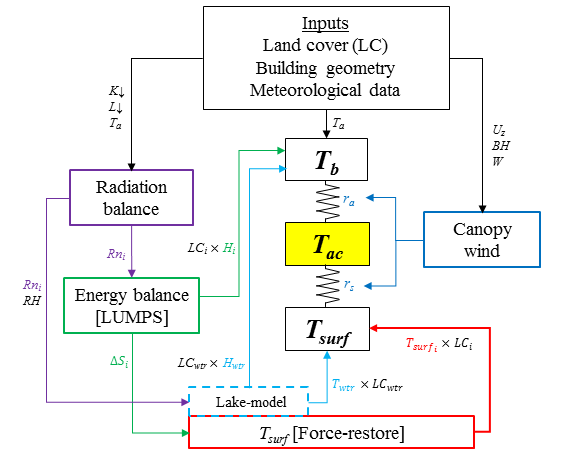
\includegraphics[trim=5mm 0mm 5mm 0mm, clip,scale=1.0]{images/Overview.png}
%}
 \caption{Overview of approach used in \glssymbol{Toolkit2} microclimate module.} \label{fig:overview}
\end{figure}

\section{Model Overview}\label{sec:ModelOverview}

\subsection{Data inputs}\label{sec:datainputs}
\subsubsection{Land cover}\label{sec:landcover}

The model uses simple data inputs, which are designed to be easily accessible. The model requires the user to define the land cover fractions of building (\glssymbol{Fbldg}), concrete (\glssymbol{Fconc}), asphalt (\glssymbol{Fasph}), grass (\glssymbol{Fgras}), irrigated grass (\glssymbol{Figrs}), tree (\glssymbol{Ftree}), and water (\glssymbol{Fwatr}). These land cover categories are self-explanatory and describe most of the surfaces in urban areas. Low vegetation (shrubs and bushes) can be included in \glssymbol{Ftree} and \glssymbol{Fbldg} collectively refers to all buildings in urban areas.  In addition to the land cover fractions, the model requires average building height (\glssymbol{BH}) and street width (\glssymbol{W}) information. These data are only needed if the user intends to calculate \glssymbol{Tac}­. In future, look up tables for these land cover variables, based on land-use or local-climate zones (LCZ) \citep{Stewart2012a} could be developed. 

\subsubsection{Meteorological data}\label{sec:metdata}

\glssymbol{Toolkit2} requires reference meteorological data to force the model. The model requires the following inputs: incoming shortwave radiation (\glssymbol{kdown}), incoming long wave radiation (\glssymbol{ldown}) (can be modelled if not available, see appendix), relative humidity (\glssymbol{RH}), reference level wind speed (\glssymbol{Uz}), and reference level air temperature (\glssymbol{Ta}).  Reference meteorological should be representative of background meteorological conditions (i.e. not significantly affected by microclimate effects).  We recommend using the nearest BoM airport weather station for reference meteorological data. BoM radiation data from a small selection of sites is freely available online\footnote{There are options available for modelling K↓, such as the Net All-wave Radiation Parameterization (NARP) of \cite{Offerle2003}, which could be integrated if needed.}.  However, other meteorological variables (\glssymbol{Ta}, \glssymbol{RH}, and \glssymbol{Uz}) are not always freely available and may need to be purchased from the BoM for a small fee. Alternatively, the CRCWSC could generate and make available reference meteorology datasets for each of Australian capital city. 

\section{Model description}\label{sec:ModelDescription}
\subsection{Net energy}\label{sec:net}

During daylight hours (\glssymbol{kdown} $\geq$ 10) net radiation (\glssymbol{Rn}) for the ith surface type is calculated using the following \citep{Loridan2011}


\begin{equation} 
\glssymbol{Rn}  
 = \glssymbol{kdown} 
 (1-\glssymbol{albedo}_{i}) +  \glssymbol{epsilon}_{i}(\glssymbol{ldown}-\glssymbol{sigma} \glssymbol{Ta}^{4}) - 0.08\glssymbol{kdown} (1- \glssymbol{albedo}_{i})) 
\label{eq:rn} \end{equation} 


where \glssymbol{albedo}$_{i}$ is \glsdesc{albedo}, \glssymbol{epsilon}$_{i}$ is \glsdesc{epsilon}, \glssymbol{Ta} is forcing air temperature (K), and \glssymbol{sigma} is the \glsdesc{sigma}. The \glssymbol{albedo}$_{i}$ and \glssymbol{epsilon}$_{i}$ values are predefined for each surface (see  Table 2.1 (TODO LABEL), validation report).  The right hand side of the equation accounts for net longwave radiation, and \glssymbol{lup} is approximated using \glssymbol{Ta}. \cite{Loridan2011}. include the term 0.08\glssymbol{kdown}$(1-\glssymbol{albedo}_{i})$ to account for the difference between near surface \glssymbol{Ta} and \glssymbol{Tsurf}. However, currently there is no correction for this difference at night. As such, we substitute Ta for. The modelled \glssymbol{Tsurf} (from 2 time steps (t) previous) is used to calculate L↑ at night. It is necessary to use  due to the method used to calculate the storage heat flux (eq. \ref{eq:ohm}), which requires \glssymbol{Rn} from the previous time step.  Testing suggests this lag does not significantly affect calculations when a 30 minute time step is used. Thus, at night (\glssymbol{kdown} $<$ 10) net radiation for i surface type is

\begin{equation} 
\glssymbol{Rn}  
 = \glssymbol{kdown} 
 (1-\glssymbol{albedo}_{i}) + \glssymbol{epsilon}_{i}] \big(\glssymbol{ldown}-\glssymbol{sigma} T_{surf[t-2]}^{4} \big) 
\label{eq:rn2} \end{equation} 


The \glssymbol{Rn} for each surface type is then used to calculate a surface energy balance for each surface. 
\subsection{Surface energy balance (LUMPS)}\label{sec:lumps}

The energy balance calculations are based on the Local-scale Urban Meteorological Parameterisation Scheme (LUMPS) \citep{Grimmond2002a}. For non-water surfaces, the sensible (\glssymbol{H}) and latent (\glssymbol{LE}) heat fluxes for the $i$th surface type are calculated using


\begin{equation} 
\glssymbol{H}_{i} = 
\frac{(1-\glssymbol{pm}_{i})+(\frac{\glssymbol{gamma}}{\glssymbol{s}})}{1+\frac{\glssymbol{gamma}}{\glssymbol{s}}}
(R_{n,i} -\Delta S_{i})- \glssymbol{beta}
\label{eq:Hi} \end{equation} 

\begin{equation} 
\glssymbol{LE}_{i} = 
\frac{\glssymbol{pm}_{i}}{1+\frac{\glssymbol{gamma}}{\glssymbol{s}}}
(R_{n,i}-\Delta S_{i})+ \glssymbol{beta}
\label{eq:LE} \end{equation} 

where \glssymbol{s} is the slope of the saturation vapour pressure-versus-temperature curve, \glssymbol{gamma} is the psychrometric constant and \glssymbol{pm}$_{i}$ and \glssymbol{beta} are based on a simplification of the Penman–Monteith approach, which takes into account the Priestley-Taylor coefficient; \glssymbol{pm}$_{i}$ depends on the surface moisture status, and \glssymbol{beta} is an empirical constant, set to 3 W m$^{-2}$ \citep{Grimmond2002a}. By default, the \glssymbol{pm} parameter is set using values from \cite{Hanna1992} (Table \ref{tab:surftype}). Alternatively, \glssymbol{pm} for vegetated classes can be defined as a function of stomatal resistance (sr) using $\glssymbol{pm} = 6.9\times10^{-6} sr^{2} - 0.004 sr + 1.3$ \citep{DeBruin1983}.  

The objective hysteresis model (OHM) is used to calculate storage heat flux for the $i$th land cover class  \citep{Grimmond2002a} 

\begin{equation} 
\Delta S_{i} = R_{n,i} a_{1,i} + \Big( \frac{\partial R_{n,i}}{\partial t}   \Big)a_{2,i} + a_{3,i}
\label{eq:ohm} \end{equation} 


where the three coefficients \glssymbol{a1}, \glssymbol{a2}, and \glssymbol{a3}, are defined for each surface (see examples in Table 2.1 TODO REFERENCE - validation report), and $\frac{\partial R_{n,i}}{\partial t} =0.5(R_{n,it-1} - R_{n,it+1})$  .  The $\Delta S_{i}$ is then used to calculate the surface temperature using the `force-restore' method.


\subsection{Surface temperature calculation (`force-restore')}\label{sec:tsurf}

The change in surface temperature \glssymbol{Tsurf} for surface $i$ with respect to time (t) is calculated as

\begin{equation} 
\frac{\partial T_{surf,i}}{\partial t}= \frac{\Delta S_{i}}{C_{i} D} - \frac{2 \pi}{\tau} (T_{surf,i -1} - T_{m,it-1})
\label{eq:force} \end{equation} 

Where $C_{i}$ is the \glsdesc{C}, $\tau$ is the period (86400 seconds), $D = 2 \glssymbol{kappa} _{i}  / \omega 0.5$, $\glssymbol{kappa} _{i}$ is the \glsdesc{kappa}, and $\glssymbol{kappa} = 2\pi / \tau$.  The first term on the right-hand side is the forcing term that affects \glssymbol{Tsurf}, while the second term is the restore term which dampens the forcing term. The \glsdesc{Tm} ($T_{m,i}$) is calculated using

\begin{equation} 
\frac{\partial T_{m,i}}{\partial t} = \frac{\Delta S_{i}}{C_{i} D_{y}}
\label{eq:tm} \end{equation} 

where \glssymbol{Dy} = $D \sqrt{365}$, the \glsdesc{Dy}. 

Thus for each time step, the aggregated \glssymbol{Tsurf} and \glssymbol{H} are equal to

\begin{equation} 
\glssymbol{H} = \sum_{i=1}^{6} (F_{i} H_{i}) + (F_{wtr} H_{wtr})
\label{eq:H} \end{equation} 

\begin{equation} 
\glssymbol{Tsurf} = \sum_{i=1}^{6} (F_{i} T_{surf,i}) + (F_{wtr} T_{wtr})
\label{eq:tsurf} \end{equation} 

As the force-restore method cannot be applied to water, we use a simple a simple water body model to calculate $H_{wtr}$ and $T_{wtr}$.


\subsection{Simple water body model}\label{sec:simplewater}

The water model in the toolkit is based on a single water layer, overlaying a soil layer. Essentially, the force-restore surface temperature model is implemented, and is overlain by a homogeneous mixed water layer (i.e. neglecting thermal stratification) representing a water body of depth z(m). The model is designed to apply to water bodies of 0.1-1.0m depths. The water model is based on the pan evaporation model of \cite{MolinaMartinez2006} which closely follows that of the lake model of \cite{Jacobs1998}. The water body model also determines the surface energy balance of the water surface. The energy balance model for the water layer is given by \citep{MolinaMartinez2006}

\begin{equation} 
\glssymbol{Sab} + \glssymbol{l*} + H_{wtr} - LE_{wtr} - \glssymbol{Gwtr} -\glssymbol{deltaSwtr} = 0
\label{eq:sab} \end{equation} 


where \glssymbol{Sab} is \glsdesc{Sab}, \glssymbol{l*}, the \glsdesc{l*}, \glssymbol{Gwtr} is the \glsdesc{Gwtr}, and \glssymbol{deltaSwtr} is the \glsdesc{deltaSwtr}. Solar radiation penetrates the water surface and is absorbed as described by Beer's Law \citep{MolinaMartinez2006}

\begin{equation} 
\glssymbol{Sab} = \glssymbol{k*} \big[ \glssymbol{betak} + (1 - \glssymbol{betak}) )(1-e^{-\glssymbol{eta}})  \big]
\label{eq:sab2} \end{equation} 

where \glssymbol{k*} is the \glsdesc{k*}, \glssymbol{betak} is the \glsdesc{betak} \citep{MolinaMartinez2006}, and \glssymbol{eta} the \glsdesc{eta}. Here, \glssymbol{eta} is given the following from \cite{Subin2012a}, for the water layer with depth z(m)

\begin{equation} 
\glssymbol{eta} = 1.1925z^{-0.424}
\label{eq:eta} \end{equation} 


A correction factor for the solar path length zenith angle is often applied to Eq. \ref{eq:sab2} \citep{MolinaMartinez2006} but this has been omitted to reduce complexity. The convective heat transport \glssymbol{Gwtr} into the soil at the base of the water layer is given by \citep{MolinaMartinez2006}

\begin{equation} 
\glssymbol{Gwtr} = - \glssymbol{Cwtr} \glssymbol{kwtr} \frac{\Delta T}{\Delta z}
\label{eq:gwtr} \end{equation} 


where \glssymbol{Cwtr} is the \glsdesc{Cwtr}, \glssymbol{kwtr} is the \glsdesc{kwtr}, 
and the change in depth $\Delta z = z$ (the depth of the water layer), the change in temperature $\Delta T$ (\degreeC) is the difference between the water temperature \glssymbol{Twtr} (\degreeC) and the soil temperature \glssymbol{Ts} (\degreeC). These initial temperatures (\glssymbol{Twtr} and \glssymbol{Ts}) must be specified (at time t = 0, they can be set to the same value). \glssymbol{kwtr} is a complex function accounting for thermal stratification and surface friction velocity. Again, to reduce complexity and assuming a mixed homogeneous water layer, a constant \glssymbol{kwtr} has been selected based on shallow lakes reported in \cite{SalasDeLeon2016} (Table \ref{tab:eddydiff}).


The latent heat flux ($LE_{wtr}$) (W m$^{-2}$) is given by \citep{Arya2001}

\begin{equation} 
LE_{wtr} = \glssymbol{rhov} \glssymbol{Lv} \glssymbol{hv} \glssymbol{Uz} (\glssymbol{qs} - \glssymbol{qa})
\label{eq:lewtr} \end{equation} 


where \glssymbol{rhov} is the \glsdesc{rhov}, \glssymbol{Lv} is the \glsdesc{Lv}, \glssymbol{hv} is the \glssymbol{hv} \citep{Jones2005,Hicks1972}, \glssymbol{Uz}, the BoM reference wind speed, \glssymbol{qs} the saturated specific humidity at $T_{wtr}$, and \glssymbol{qa} is the specific humidity of the air at \glssymbol{Ta} (see appendix for calculation of \glssymbol{rhov}, \glssymbol{qs} and \glssymbol{qa}). The sensible heat flux is given by \cite{MolinaMartinez2006}\footnote{The temperature gradient (\glssymbol{Ta}-\glssymbol{Ts}) in Eq. 6 from \cite{MolinaMartinez2006} pg. 254 is reversed here from the usual (\glssymbol{Ts}-\glssymbol{Ta}). It accounts for the addition of sensible heat to the water layer from the energy balance equation (Eq. \ref{eq:rn}).}

\begin{equation} 
H_{wtr} = \glssymbol{rhoa} \glssymbol{cp} \glssymbol{hc} \glssymbol{Uz} (\glssymbol{Ta}-\glssymbol{Ts})
\label{eq:hwtr} \end{equation} 

where \glssymbol{rhoa} is the \glsdesc{rhoa}, \glssymbol{cp} the \glsdesc{cp}, and \glssymbol{hc} the \glsdesc{hc}. Returning to Eq. \ref{eq:sab2}, net long wave radiation \glssymbol{l*} = \glssymbol{Rn} - \glssymbol{k*} leaving $\Delta S_{wrt}$ from the energy balance equation, which is defined as \citep{MolinaMartinez2006}

\begin{equation} 
\Delta S_{wrt} = \glssymbol{Cwtr} z \frac{\Delta T_{wtr}}{\Delta t}
\label{eq:swrt} \end{equation}



where $\Delta t$ is change in time (seconds) and \glssymbol{Cwtr} is the \glsdesc{Cwtr}. Solving for $\Delta T_{wtr}$ and adding the change in temperature to the previous time step ($T_{wtr} = T_{wtr,t-1}  + \Delta T_{wtr}$) gives the new water layer temperature. 


Below the water layer, the Force-Restore model (Eq. \ref{eq:force}) determines the soil surface temperature where \glssymbol{Gwtr} is equivalent to $\Delta S_{i}$  for other surfaces. The soil layer parameters are set to saturated soil where the volumetric heat capacity is set to \glssymbol{C} $= 3.03 \times 10^{6}$ (J m$^{-2}$ K$^{-1}$) and the thermal diffusivity is set to \glssymbol{kappa} $= 0.625 \times 10^{-6}$ (m$^{2}$ s$^{-1}$). 


\subsection{Calculation of urban canopy layer air temperature (\glssymbol{Tac}) }\label{sec:calcTac}


The \glssymbol{Tac} term is calculated following the approach outlined in Figure \ref{fig:Tac}. 


\begin{figure}[!htbp]
%\fbox{
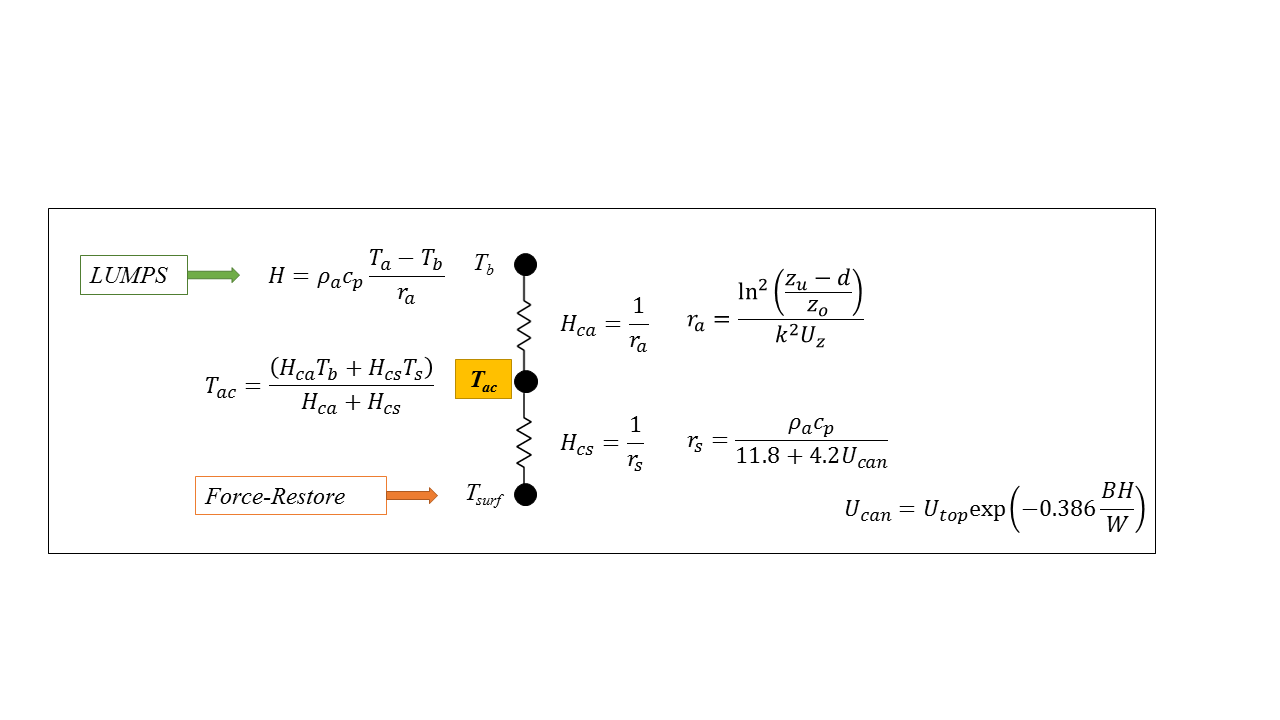
\includegraphics[trim=13mm 43mm 32mm 55mm, clip,scale=0.60]{images/Tac.png}
%}
 \caption{Schematic of the air temperature module.} \label{fig:Tac}
\end{figure}


First we, solve the following equation for \glssymbol{Tb} (Yang et al 2011 TODO FIND THIS REFERENCE). This assumes a generic local scale \glssymbol{Ta} for the site (all grid cells). 

\begin{equation} 
H = \glssymbol{rhoa} \glssymbol{cp} \frac{\glssymbol{Ta}-\glssymbol{Tb}}{\glssymbol{ra}}
\label{eq:H_air} \end{equation}

where \glssymbol{cp} is the \glsdesc{cp} and \glssymbol{rhoa} is the \glsdesc{rhoa}. 

The canopy to atmosphere resistance (\glssymbol{ra}) is given by (Yang et al 2011 TODO FIND THIS REFERENCE):

\begin{equation} 
\glssymbol{ra} = \frac{ln^{2} \Bigg( \frac{\glssymbol{zu}-\glssymbol{d}}{\glssymbol{z0}}   \Bigg)   } {k^{2} \glssymbol{Uz}}
\label{eq:ra} \end{equation}

Where \glssymbol{zu} is the \glsdesc{zu}, \glssymbol{d} is the \glsdesc{d}, and \glssymbol{z0} is the \glsdesc{z0}. 


The temperature of the canopy layer (\glssymbol{Tac}) is then given by \citep{Oleson2010} 

\begin{equation} 
\glssymbol{Tac} = \frac{\glssymbol{Hca} + \glssymbol{Tb} + \glssymbol{Hcs} + \glssymbol{Tsurf} }  { \glssymbol{Hca}  + \glssymbol{Hcs} }
\label{eq:tac} \end{equation}

which is a simplification of Equation 3.75 (eq. \ref{eq:clmu375}) in the CLMU technical note \citep{Oleson2010}:, because we do not consider sensible heat conductance for individual surface types. Sensible heat conductance are given for the urban canopy layer to atmosphere (\glssymbol{Hca}) and surface to urban canopy layer (\glssymbol{Hcs}) by \citep{Oleson2010}



\begin{equation} 
\glssymbol{Hca} = \frac{1}{\glssymbol{ra}} \glssymbol{Hcs} = \frac{1}{\glssymbol{rs}}
\label{eq:hca} \end{equation}

where \glssymbol{rs} is the \glsdesc{rs}

\begin{equation} 
\glssymbol{rs} = \frac{\glssymbol{rhoa}\glssymbol{cp}}{11.8+4.2\glssymbol{Ucan}}
\label{eq:rs} \end{equation}
 				
\glssymbol{Ucan} is the \glsdesc{Ucan}


\begin{equation} 
\glssymbol{Ucan} = \glssymbol{Utop} exp{ \Bigg( -0.386 \frac{\glssymbol{BH}}{\glssymbol{W}} \Bigg)}
\label{eq:ucan} \end{equation}

where \glssymbol{Utop} is the \glsdesc{Utop}, \glssymbol{BH} is the \glsdesc{BH} and \glssymbol{W} is the \glsdesc{W}. \glssymbol{Utop} is estimated at the top of the UCL based on \glssymbol{Uz} using a logarithmic relationship:




\begin{equation} 
\glssymbol{Utop} = \glssymbol{Uz} \frac{ ln \big( \frac{\glssymbol{BH}}{\glssymbol{z0}}  \big)}{ ln \big( \frac{\glssymbol{zu}}{\glssymbol{z0}}  \big) }
\label{eq:xx4} \end{equation}

If \glssymbol{BH} is below the domain average building height, it should be set to the domain average. 

\section{Model validation}\label{sec:validation}
\subsection{Overview}\label{sec:validationover}



This paper provides a validation of the new microclimate model for the CRCWSC toolkit (hereafter referred to as \glssymbol{Toolkit2}). \glssymbol{Toolkit2} aims to calculate surface temperature (\glssymbol{Tsurf}) and surface level (urban canopy layer) air temperature (\glssymbol{Tac}) in urban areas using simple and well-known urban climate modelling methods. The model is primarily intended to calculate the cooling benefits of water sensitive urban design (WSUD) during hot and sunny summertime conditions. For a full description of \glssymbol{Toolkit2} see the technical document attached. For this validation we draw upon a range of data from Melbourne and Adelaide to test \glssymbol{Tsurf} and \glssymbol{Tac} calculations. 

\subsection{Methods and data}\label{sec:methods}
\subsubsection{Introduction}\label{sec:methodsintro}

As part of the validation we conducted a range of simulations that test model performance for both \glssymbol{Tsurf} and \glssymbol{Tac}. These validation experiments are focussed on summertime conditions.  Firstly, we conducted detailed testing of model performance at simulating \glssymbol{Tsurf} for each land cover class that can be prescribed in \glssymbol{Toolkit2} (i.e. dry grass, asphalt etc.), using ground-based observations of \glssymbol{Tsurf} (section \ref{sec:landcoversim}). These simulations by land cover type, provide a detailed assessment of model parameters, and the underlying energy balance dynamics and resulting \glssymbol{Tsurf} for each land cover class. Secondly, we conducted suburb scale simulations of Mawson Lakes, Adelaide, for which we have high resolution remotely sensed \glssymbol{Tsurf} observations and in situ \glssymbol{Tac} data (section \ref{sec:suburbsim}).  The suburb scale simulations reflect the way the model is intended to be operationalised by practitioners.

\subsubsection{Land cover simulations}\label{sec:landcoversim} 

To test model performance at simulating \glssymbol{Tsurf} of different land cover classes, and check a number of model parameters we utilised ground-based observations of \glssymbol{Tsurf} from the Melbourne metropolitan area. \cite{Coutts2016a} deployed infrared temperature sensors (SI-121 - Apogee), during February 2012, across a range of land cover types including: asphalt, concrete, grass, irrigated grass, steel roof, and water. The conditions during this period represented near-typical summertime conditions in Melbourne; including a number of days (15th, 24th, and 25th February) where air temperature exceeded 30\degreeC (see Figure \ref{fig:met}). These hotter days were characterised by northerly winds, which bring hot and dry air from Australia's interior, and often result in heatwave conditions in Melbourne. Additionally, there was at least one cloudy day where incoming shortwave radiation (\glssymbol{kdown}) dropped significantly and negligible amount of rainfall occurred (16th February).  In addition, to assess tree \glssymbol{Tsurf} we obtained a different set of observational data from the Monash cemetery tree experiment \citep{Coutts2016b}, including \glssymbol{Tsurf} observations of the tree canopy (collected during February 2014). We also obtained a BoM meteorological forcing data for the 2014 case study period.  This period (not shown) was very similar to the February 2012 period, with typical summer days punctuated by hotter and drier northerly conditions. 

\begin{figure}[!htbp]
%\fbox{
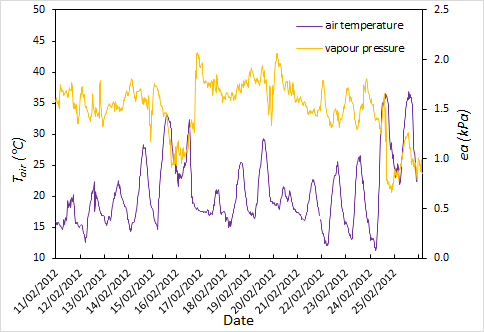
\includegraphics[trim=0mm 0mm 0mm 0mm, clip,scale=0.65]{images/met1.png}
~
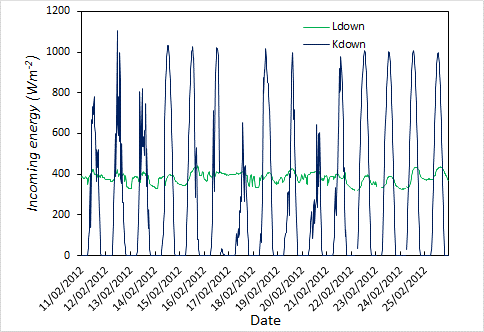
\includegraphics[trim=0mm 0mm 0mm 0mm, clip,scale=0.65]{images/met2.png}
%}
 \caption{Meteorological conditions during land cover validation period. Data source: Melbourne Airport Bureau of Meteorology (ID 086282) weather station.} \label{fig:met}
\end{figure}


The model was run for each of the 7 land cover types, and was forced with hourly data from Melbourne Airport Bureau of Meteorology (ID 086282) weather station data (Figure 2.1).  The following data were used as inputs: reference air temperature (\glssymbol{Ta}), incoming shortwave radiation (\glssymbol{kdown}), incoming long wave radiation (\glssymbol{ldown}), and relative humidity ($RH$). The model was spun up for 24 hours, although testing suggests minimal spin up is required. Initial conditions for average ground temperature (\glssymbol{Tm}) were obtained via Jacobs et al. (2000) TODO FIND REFERENCE and sensitivity testing. The model parameter setup is summarised in Table \ref{tab:Parameter}. As \glssymbol{Tac} was not calculated for these simulations we did not require wind speed or building height and street width information. 



\begin{table}[!htbp]
\caption{Parameter setup for all \glssymbol{Toolkit2} simulations in this report.}  
\label{tab:Parameter}
  \begin{tabular}{  | p{2.5cm} | p{1.5cm} |p{1.5cm} |p{1.5cm} |p{1.5cm} |p{1.5cm} |p{1.5cm} |p{1.5cm} |p{1.5cm} |} 
	\hline  \textbf{ } & \textbf{Roof} & \textbf{Asphalt}& \textbf{Water}& \textbf{Water}& \textbf{Concrete}& \textbf{Tree}& \textbf{Dry grass}& \textbf{Irrigated grass} \\ 	
	 \textbf{ } & \textbf{} & \textbf{}& \textbf{Water}& \textbf{Soil}\footnote{soil layer beneath water}& \textbf{}& \textbf{}& \textbf{ }& \textbf{ } \\ \hline	
Albedo (\glssymbol{albedo}) & 0.15 & 0.08 &0.1 &N/A &0.2 &0.1 &0.19 &0.19 \\ \hline
Emissivity (\glssymbol{epsilon})&0.90&0.95&0.97&N/A&0.94&0.98&0.98&0.98\\ \hline
Heat capacity ($C$) ($\times10^{6}$) &0.09&1.94&4.18&3.03 &2.11&2.55&1.35&2.19\\ \hline
Thermal diffusivity ($\times10^{-6}$)&19.17&0.38&0.14&0.63&0.72&0.42&0.21&0.42\\ \hline	
Ground temperature initial (\glssymbol{Tm}) (\degreeC)\footnote{bracketed values were used in second Mawson Lakes suburb simulation - derived from 1 month spin-up} &25.0&26.0&25.0&25.0&26.0&20.0&20.0&20.0\\ 
&(28.2)&(29.0)&(24.5)&(24.5)&(27.9)&(20.8)&(22.4)&(21.5) \\ \hline
OHM [\glssymbol{a1}, \glssymbol{a2}, \glssymbol{a3}]&[0.12,0.24,-4.5]&[0.36,0.23,-19.3] &N/A &N/A&[0.67,0.31,-31.45]&[0.11,0.11,-12.3]&[0.21,0.11,-16.10]&[0.32,0.54,-27.40] \\ \hline
Alpha Penman-Monteith (\glssymbol{pm}) \cite{Hanna1992}&0.0&0.0&N/A&N/A&0.0&1.0&0.2&1.0 \\ \hline
Beta coefficient (\glssymbol{beta}) (W m$^{-2}$) \cite{Grimmond2002a}&3&3&3&3&3&3&3&3 \\ \hline
OHM source &`Suburban' \cite{Jarvi2014a} &Asphalt \cite{Narita1984}&N/A&N/A&Asphalt \cite{Narita1984} and \cite{Asaeda1993} &`Mixed forest' \cite{McCaughey1985} &`Unirrigated grass' \cite{Grimmond1993}&`Short grass' \cite{Doll1985} \\ \hline
Thermal properties source &Average  of concrete (11.6 mm), air (1000 mm), wood (40 mm), and plasterboard (12.5 mm) &\cite{Oke1987z} &\cite{Oke1987z} &\cite{Oke1987z} &\cite{Oke1987z}  &\cite{Moore1986} &Average dry sand +clay soils \cite{Oke1987z} &Average of wet + dry sand + clay \cite{Oke1987z} \\ \hline	
  \end{tabular} 
\end{table}



\subsubsection{Suburb scale simulations (Mawson Lakes)}\label{sec:suburbsim} 
 
In addition to the land cover category testing, we also conducted suburb scale simulations of \glssymbol{Tsurf} and \glssymbol{Tac} for Mawson Lakes, Adelaide (Figure \ref{fig:mawson}). The suburb scale simulations utilised observational data from the Mawson Lakes field campaign, conducted 13-18th February 2011, which represented average summertime conditions in Adelaide. For these simulations the model was run on a 30m grid over the Mawson Lakes suburb for the period 13th-18th February (Figure \ref{fig:met3}).  Remotely sensed land cover data from the campaign (see Figure \ref{fig:mawson} - right) were used to define land cover, and building height to width ratio was defined using LiDAR data \citep{Broadbent2016}. The Mawson Lakes simulations used the same parameter setup as above (summarised in Table \ref{tab:Parameter}), and were forced with meteorological data from the Kent Town Bureau of Meteorology (ID 023090) weather station. Modelled \glssymbol{Tsurf} was validated using remotely sensed ­\glssymbol{Tsurf} (night - 15th February and day - 16th February), which was resampled to 30 m resolution. To validate \glssymbol{Tac} we utilised data from 27 automatic weather station (AWS), which were also deployed during the Mawson Lakes field campaign (see Figure \ref{fig:mawson} for AWS locations). 
 


\begin{figure}[!htbp]
%\fbox{
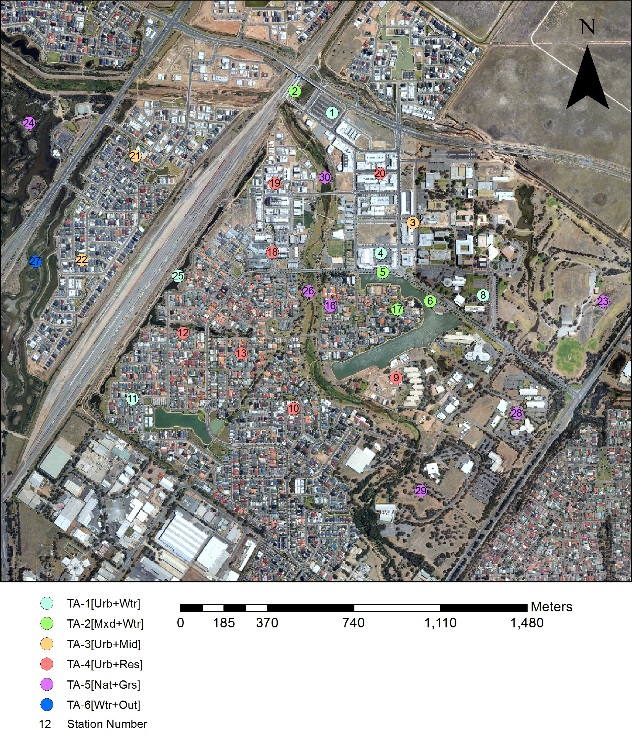
\includegraphics[trim=0mm 0mm 0mm 0mm, clip,scale=1.25]{images/Mawson1.jpg}
~
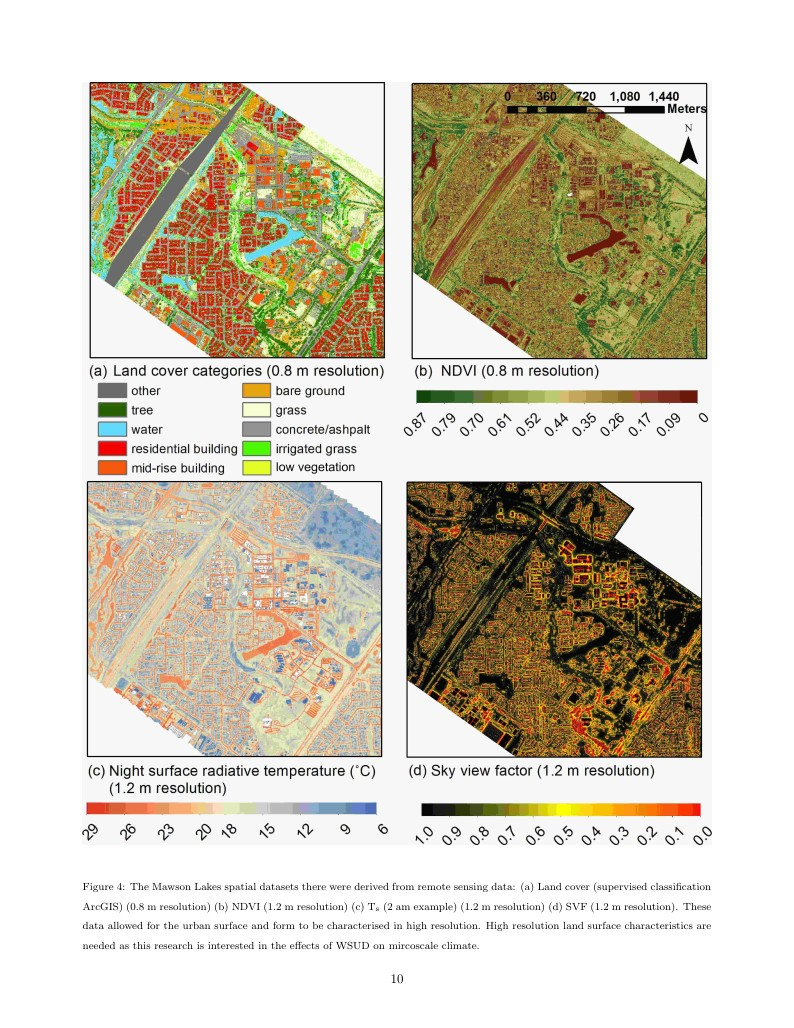
\includegraphics[trim=30mm 194mm 142mm 28mm, clip,scale=0.78]{images/Mawson2.png}
%}
 \caption{Mawson Lakes suburb: weather station locations (left) and land cover data (right) \citep{Broadbent2016}.} \label{fig:mawson}
\end{figure}


\begin{figure}[!htbp]
%\fbox{
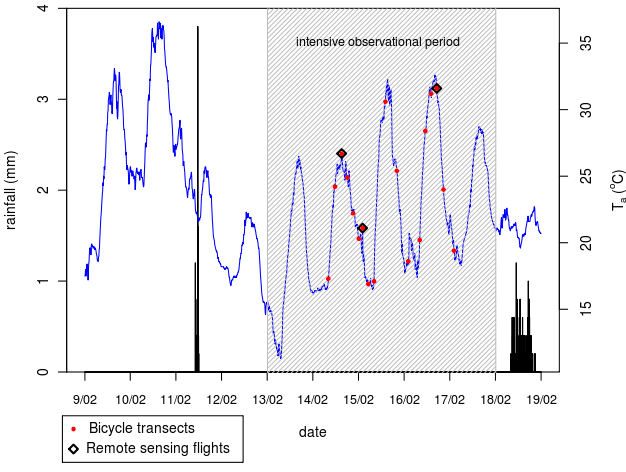
\includegraphics[trim=0mm 0mm 0mm 0mm, clip,scale=1.0]{images/met3.png}
%}
 \caption{Meteorological condition during the Mawson Lakes field campaign \citep{Broadbent2016}.} \label{fig:met3}
\end{figure}


\subsection{Results}\label{sec:Results} 
\subsubsection{Land cover simulations}\label{sec:landcoverresult} 


The \glssymbol{Tsurf} for each land cover class was simulated for a 14 day period during February 2012. The modelled \glssymbol{Tsurf} for all 3 impervious surfaces (roof, asphalt, and concrete) were reasonably well predicted with root-mean-square-errors (RMSE) of 5.16, 4.66, and 4.08\degreeC, respectively (Figures \ref{fig:roofobs}, \ref{fig:concreteobs}, and \ref{fig:asphaltobs}).  Roof and concrete \glssymbol{Tsurf} was generally slightly over-predicted at night (lower \glssymbol{Tsurf}) and under-predicted at the daily maxima (higher \glssymbol{Tsurf}); these patterns are commonly observed in other land surface models.  For asphalt, \glssymbol{Tsurf} was generally over-predicted at all temperatures. The night of the 16 February, when overnight conditions were warm, was well captured for asphalt and rooftop locations, but not well captured at the concrete site. The concrete \glssymbol{Tsurf} was anomalously high (up to 5\degreeC warmer than the asphalt site) on the night of 16 February, which may have been caused by a strong warm air advection effect at the concrete site. This approach probably cannot account for the effects of warm air advection on \glssymbol{Tsurf}. Nevertheless, the broad timing and magnitude of heating and cooling was well captured for all the impervious land cover types. 



\begin{figure}[!htbp]
%\fbox{
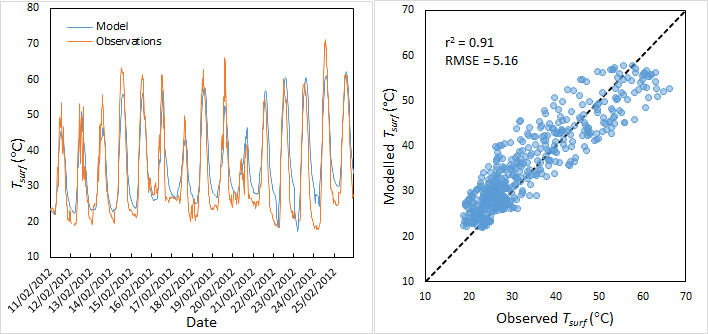
\includegraphics[trim=0mm 0mm 0mm 0mm, clip,scale=0.68]{images/roofobs.png}
%}
 \caption{Observed vs Modelled \glssymbol{Tsurf} for rooftop site.} \label{fig:roofobs}
\end{figure}


\begin{figure}[!htbp]
%\fbox{
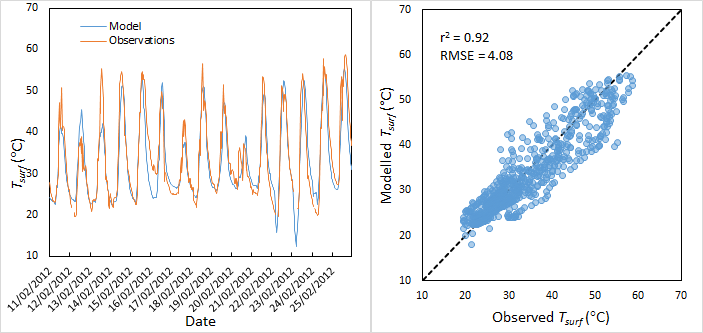
\includegraphics[trim=0mm 0mm 0mm 0mm, clip,scale=0.68]{images/concreteobs.png}
%}
 \caption{Observed vs Modelled \glssymbol{Tsurf} for concrete site.} \label{fig:concreteobs}
\end{figure}

\begin{figure}[!htbp]
%\fbox{
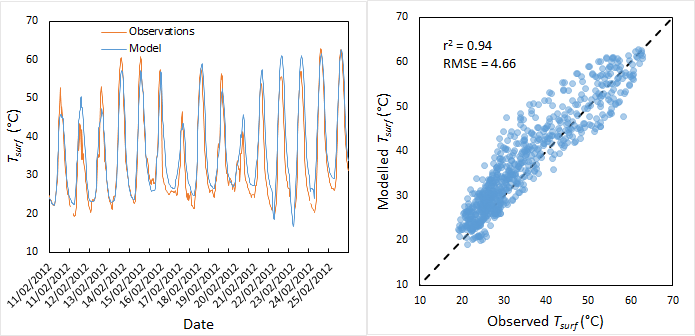
\includegraphics[trim=0mm 0mm 0mm 0mm, clip,scale=0.88]{images/asphaltobs.png}
%}
 \caption{Observed vs Modelled \glssymbol{Tsurf} for asphalt site.} \label{fig:asphaltobs}
\end{figure}
	


Irrigated grass had a lower RMSE (4.06\degreeC) than impervious surfaces, but this is partly because the amplitude of \glssymbol{Tsurf} variability was lower (Figure \ref{fig:irrgrassobs}).  By contrast, dry grass had the largest RMSE of the surfaces tested (6.26\degreeC), as dry grass had the largest amplitude of \glssymbol{Tsurf} variability (Figure \ref{fig:drygrassobs}). Further, both grass surfaces exhibited the same skewing in the scatterplot as the impervious surfaces, with a general over-prediction of night-time temperatures and under-prediction of daytime maxima. 



\begin{figure}[!htbp]
%\fbox{
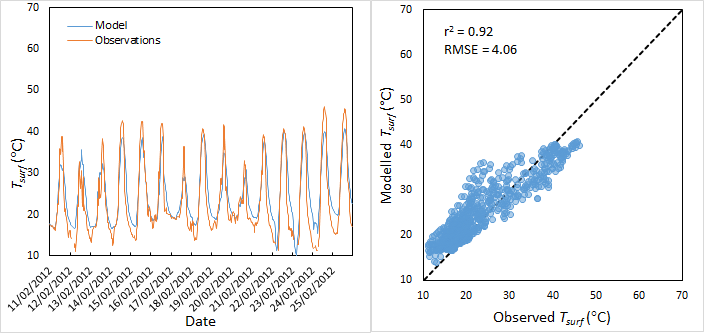
\includegraphics[trim=0mm 0mm 0mm 0mm, clip,scale=0.88]{images/irrgrassobs.png}
%}
 \caption{Observed vs Modelled \glssymbol{Tsurf} for irrigated grass site.} \label{fig:irrgrassobs}
\end{figure}

 
\begin{figure}[!htbp]
%\fbox{
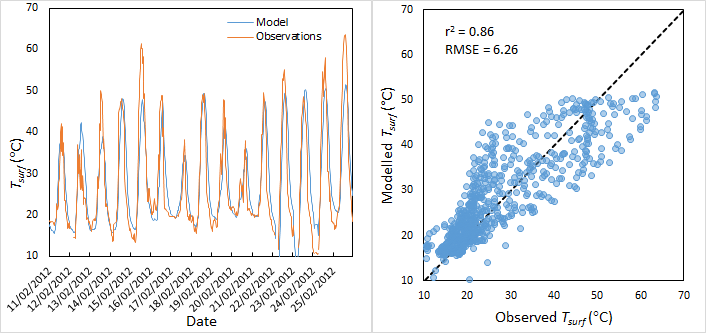
\includegraphics[trim=0mm 0mm 0mm 0mm, clip,scale=0.68]{images/drygrassobs.png}
%}
 \caption{Observed vs Modelled \glssymbol{Tsurf} for dry grass site.} \label{fig:drygrassobs}
\end{figure}



Model performance for water \glssymbol{Tsurf} had a low RMSE of 2.31\degreeC, but the $r^{2}$ value of 0.76 suggests \glssymbol{Tsurf} was predicted less accurately than other surfaces (Figure \ref{fig:waterobs}). In particular, daily maxima were under-predicted on hotter days (e.g. 14th February). \glssymbol{Toolkit2} uses a different module for water bodies (see technical notes), as the force-restore method does not work for water. This module treats water as a single layer (with depth z) overlying soil. It may be that a multi-layer water body model is needed to more accurately capture water \glssymbol{Tsurf} on hot days.  Despite the under-prediction on 14 February, the simple water body model can reproduce water \glssymbol{Tsurf} to an acceptable standard. 

The \glssymbol{Tsurf}­ of trees had the lowest $r^{2}$ suggesting that the force-restore method, which was originally designed for soil, does not work for trees (Figure \ref{fig:treeobs}). Nevertheless, the data from \cite{Coutts2016b}, suggests that reference air temperature can be used as a surrogated for tree \glssymbol{Tsurf} (Figure \ref{fig:airtreeobs}). Accordingly, tree \glssymbol{Tsurf} will be directly approximated using $T_{a}$ in the model. 




\begin{figure}[!htbp]
%\fbox{
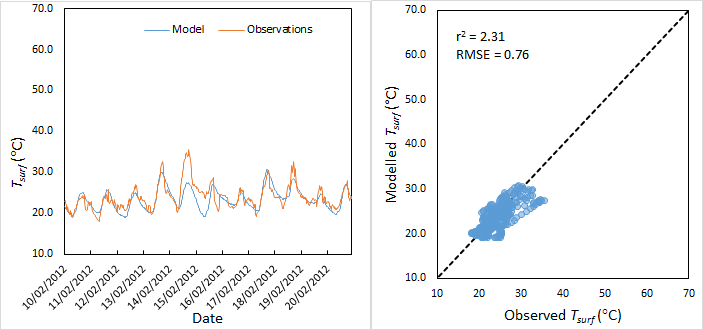
\includegraphics[trim=0mm 0mm 0mm 0mm, clip,scale=0.88]{images/waterobs.png}
%}
 \caption{Observed vs Modelled \glssymbol{Tsurf} for water site.} \label{fig:waterobs}
\end{figure}



\begin{figure}[!htbp]
%\fbox{
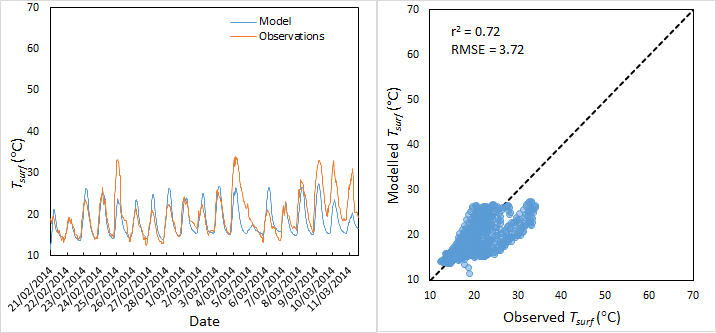
\includegraphics[trim=0mm 0mm 0mm 0mm, clip,scale=0.68]{images/treeobs.png}
%}
 \caption{Observed vs Modelled \glssymbol{Tsurf} for tree canopy site.} \label{fig:treeobs}
\end{figure}

\begin{figure}[!htbp]
%\fbox{
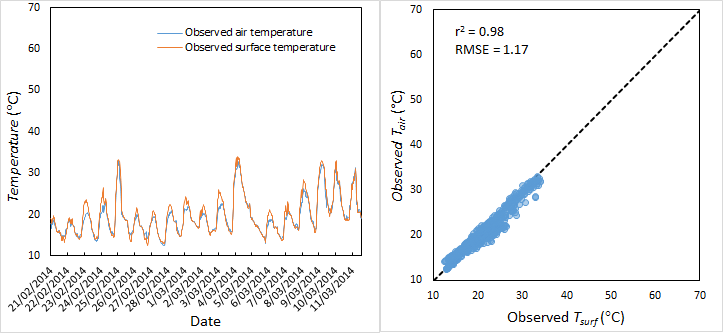
\includegraphics[trim=0mm 0mm 0mm 0mm, clip,scale=0.88]{images/airtreeobs.png}
%}
 \caption{Observed air temperature vs. observed tree \glssymbol{Tsurf}. It was found that air temperature is an accurate predictor of tree \glssymbol{Tsurf}.} \label{fig:airtreeobs}
\end{figure}


\subsubsection{Suburb scale simulations (Mawson Lakes)}\label{sec:suburbresult} 
\paragraph{Surface temperature}\label{sec:surftempresult} 



In addition to the land cover simulations (discussed above) we conducted suburb scale modelling of the Mawson Lakes suburb. These simulations reveal how the \glssymbol{Toolkit2} model could operationalised by practitioners who want to assess the cooling benefits of WSUD or greening initiatives. Suburb scale simulations were conducted using the same parameters as above (Table \ref{tab:Parameter}). Figure \ref{fig:MawsonBase} shows the predicted \glssymbol{Tsurf} (30m) for the Mawson Lakes domain plotted against observed \glssymbol{Tsurf} (30m). Firstly, the model output shows that some land cover is wrongly categorised, resulting in population of grid points where modelled \glssymbol{Tsurf} is over-predicted. Additionally, large model “errors” are caused by heterogeneity of roof emissivity may have contributed to large inaccuracies in observed roof \glssymbol{Tsurf}. 

The results suggests that, with the default setup, both day and night \glssymbol{Tsurf} were under-predicted by model. The range of modelled nocturnal \glssymbol{Tsurf} variability (c. 8\degreeC) was much smaller than observed variability (c. 18\degreeC). This under-prediction of variability could reflect the fact that some processes that dictate the rate of nocturnal cooling, including sky-view-factor and reduced longwave heat loss, are not accounted for in this approach

Model testing revealed that the initial \glssymbol{Tm} parameter is important for determining nocturnal \glssymbol{Tsurf}. Accordingly, the model was run a second time for the Mawson Lakes domain, with the initial \glssymbol{Tm} defined using a 1 month spin up (see Figure \ref{fig:MawsonSpin}). The original initial \glssymbol{Tm} values were based on assumed values for Melbourne simulations (Section \ref{sec:landcoverresult}) and were too low for Adelaide. The increased \glssymbol{Tm} significantly improves night \glssymbol{Tsurf} performance with RMSE dropping from 3.8 to 2.6\degreeC and model performance for daytime \glssymbol{Tsurf} is also improved (Figure \ref{fig:MawsonSpin}).

Overall, the model performance with increased \glssymbol{Tm} is improved, with the spatial variability and magnitude of \glssymbol{Tsurf} well captured. However, with higher \glssymbol{Tm}, the range of nocturnal \glssymbol{Tsurf} variability is still under-predicted.  There are at least two implications that arise for these simulations. Firstly, the initial conditions of the \glssymbol{Tm} parameter (which represents the average temperature in the surface layer) are very important for good model performance. It is recommended that users define \glssymbol{Tm} using a spin-up period - this function could be built into the model, but it does mean more data is required.  Secondly, the nocturnal \glssymbol{Tsurf} of impervious surfaces was also under-predicted in the land cover simulations (i.e. Section \ref{sec:landcoverresult}) under warm advection conditions. Although warm advection conditions were not observed during the Mawson Lakes campaign, it could be worthwhile further investigating this phenomenon to negate its effect and improve nocturnal \glssymbol{Tsurf} accuracy. 


\begin{figure}[!htbp]
%\fbox{
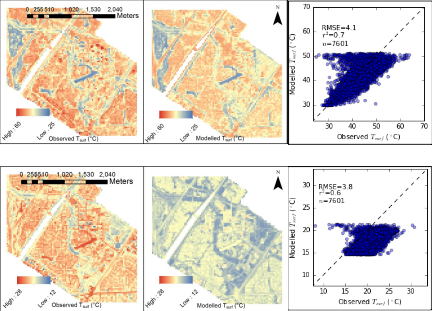
\includegraphics[trim=0mm 0mm 0mm 0mm, clip,scale=1.05]{images/MawsonBase.png}
%}
 \caption{Mawson Lakes (base run) - observed \glssymbol{Tsurf} and modelled \glssymbol{Tsurf} for day (TOP) and night (BOTTOM).} \label{fig:MawsonBase}
\end{figure}

 


\begin{figure}[!htbp]
%\fbox{
\begin{center}
\textbf{{\Large DAY (3pm 16 Feb)}}
\end{center}
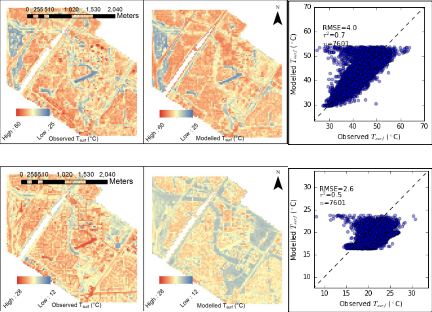
\includegraphics[trim=0mm 0mm 0mm 0mm, clip,scale=1.05]{images/MawsonSpin.png}
%}
\begin{center}
\textbf{{\Large NIGHT (3pm 16 Feb)}}
\end{center}
 \caption{Mawson Lakes (spin-up \glssymbol{Tm} run) - observed \glssymbol{Tsurf} and modelled \glssymbol{Tsurf} for day (TOP) and night (BOTTOM).} \label{fig:MawsonSpin}
\end{figure}



\paragraph{Air temperature}\label{sec:airtempresult} 


Spatial plots of modelled 3am and 3pm \glssymbol{Tac} are shown in Figure \ref{fig:MawsonModelledTas}. We also extracted modelled \glssymbol{Tac} from the grid points where the 27 AWS were located (grid points were centred at the AWS) for a 2 day period (15-16th February 2011) (Figure \ref{fig:MawsonModObs}). For the spin-up \glssymbol{Tm}, which had the best \glssymbol{Tsurf} performance (Figure \ref{fig:MawsonSpin}), the \glssymbol{Tac} was generally well predicted (Figure \ref{fig:MawsonModObs}).  The model tends to over-predict daily maximum \glssymbol{Tac} at all sites (Figure \ref{fig:MawsonBox}).  The model performed poorly at open sites with a lot of adjacent impervious surfaces (e.g. a carpark - station 1), where \glssymbol{Tac} was significantly over-predicted (this can also be seen in the Figure \ref{fig:MawsonModelledTas}).  This over-prediction could occur because daytime \glssymbol{Tsurf} was slightly over-predicted (Figure \ref{fig:MawsonSpin}), or because canyon wind speed (\glssymbol{Ucan}) was over-predicted (Figure \ref{fig:MawsonUcan}). However, simulations with observed \glssymbol{Ucan} (not shown) produced very similar \glssymbol{Tac} results, suggesting the problem relates to \glssymbol{Tsurf} and the sensible heat flux ($H$).  




\begin{figure}[!htbp]

\begin{center}
\textbf{{\Large NIGHT (3am 15 Feb)}} ~~~~~~~~~~~~~~~~~~~~~~~~~~~~~~~ \textbf{{\Large DAY (3pm 16 Feb)}}
\end{center}
%\fbox{
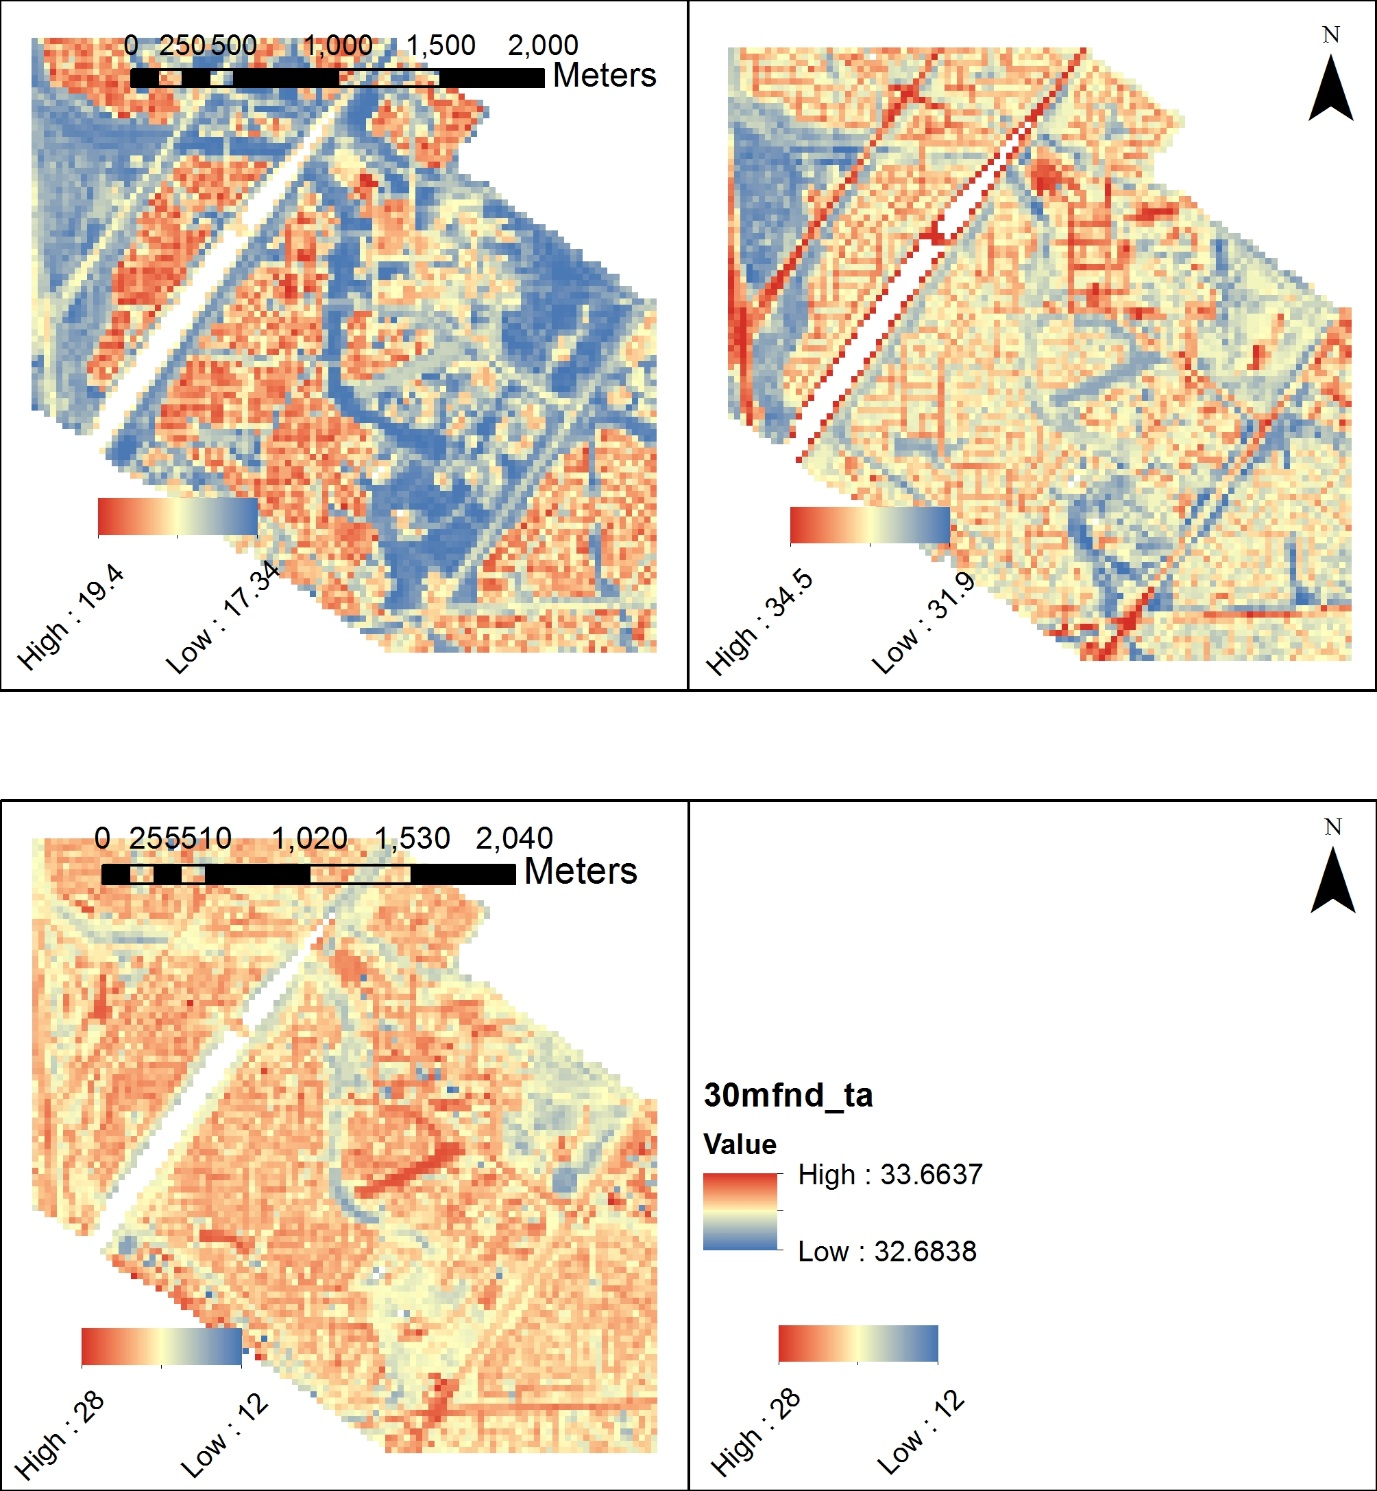
\includegraphics[trim=0mm 92mm 0mm 0mm, clip,scale=1.05]{images/MawsonModelledTas.jpg}
%}
 \caption{Modelled $T_{ax}$ for night (3 am) and day (3 pm) in Mawson Lakes domain (increased \glssymbol{Tm} run).} \label{fig:MawsonModelledTas}
\end{figure}


The model also under-predicts nocturnal $T_{ax}$ at natural sites (e.g. station 23, golf course), and this may occur because grass \glssymbol{Tsurf} was under predicted at night. The model does not account for changes in atmospheric stability, which can significantly influence exchanges of heat between the atmosphere and the UCL, especially at night.  

Overall, the general trends in spatial and temporal variability are well captured given the simplicity of the approach used. The toolkit out-performed a more complicated and computationally demanding land surface model, SURFEX \citep{Masson2013}, for \glssymbol{Tac} simulations at Mawson Lakes. 




\begin{figure}[!htbp]
%\fbox{
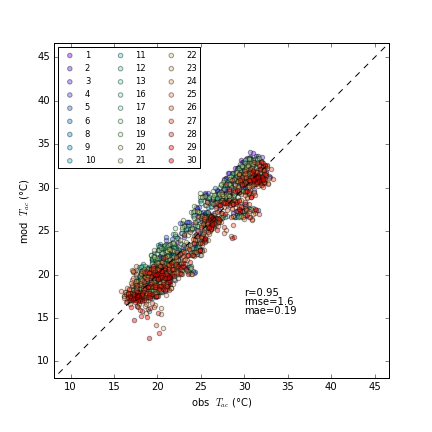
\includegraphics[trim=0mm 0mm 0mm 0mm, clip,scale=1.0]{images/MawsonModObs.png}
%}
 \caption{Mawson Lakes (spin-up \glssymbol{Tm} run) - Modelled \glssymbol{Tac} vs observed \glssymbol{Tac} for 15-16th February 2011 (30 minute data).} \label{fig:MawsonModObs}
\end{figure}

\begin{figure}[!htbp]
%\fbox{
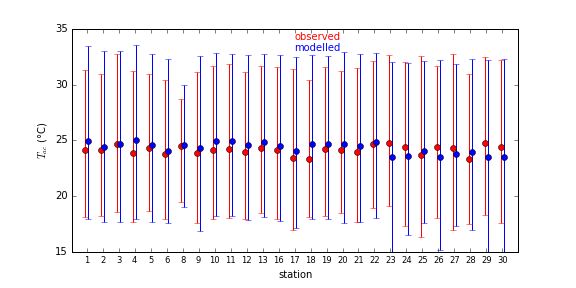
\includegraphics[trim=0mm 0mm 0mm 0mm, clip,scale=0.8]{images/MawsonBox.png}
%}
 \caption{Mawson Lakes (spin-up \glssymbol{Tm} run) - boxplot of modelled \glssymbol{Tac} (blue) vs observed \glssymbol{Tac} (red) with average, min, and max $T_{ax}$ shown. Boxplots were generated from 30 minute data from period 15-16th February 2011.} \label{fig:MawsonBox}
\end{figure}





\begin{figure}[!htbp]
%\fbox{
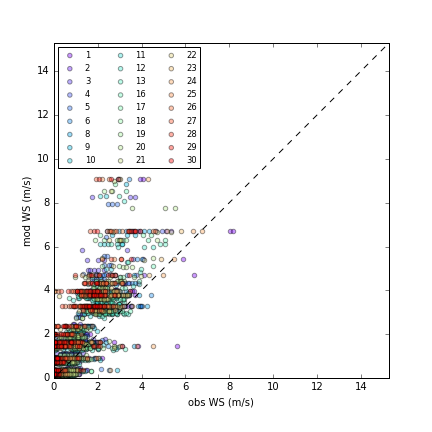
\includegraphics[trim=0mm 0mm 0mm 0mm, clip,scale=1.0]{images/MawsonUcan.png}
%}
 \caption{Mawson Lakes (increased \glssymbol{Tm} run) - Modelled \glssymbol{Ucan} vs observed \glssymbol{Ucan}.} \label{fig:MawsonUcan}
\end{figure}


































\section{Code availability}\label{sec:available}

\printglossary[title={List of Symbols}]

\section*{Acknowledgements}
The support of the Commonwealth of Australia through the Cooperative Research Centre program is acknowledged.
%\end{acknowledgements}

\section*{References}\label{sec:ref}
%% If you have bibdatabase file and want bibtex to generate the
%% bibitems, please use
%%
  \bibliographystyle{elsarticle-harv} 
  \bibliography{library}

%% else use the following coding to input the bibitems directly in the
%% TeX file.

\begin{thebibliography}{00}

%% \bibitem[Author(year)]{label}
%% Text of bibliographic item

\bibitem[ ()]{}

\end{thebibliography}


%% The Appendices part is started with the command \appendix;
%% appendix sections are then done as normal sections
\appendix
\setcounter{table}{0}
\renewcommand{\thetable}{A\arabic{table}}

%\subsection{}                               %% Appendix A1, A2, etc.


%%%%%%%%%% taking out parameterizations
\section{Appendix}\label{sec:app}  
\subsection{Additional data tables}\label{app:tables}  


\begin{table}[!htbp]
\caption{Previously quoted values for \glssymbol{pm}: range listed by \cite{Hanna1992} based on information presented by \cite{Beljaars1991}.}  
\label{tab:surftype}
  \begin{tabular}{   c  c } 
	\hline  \textbf{Surface type} & \textbf{pm}  \\ \hline
	Dry desert with no rain for months & 0.0 - 0.2   \\ 
	Arid rural area & 0.2 - 0.4    \\ 
	Crops and field, midsummer (minimal rain) & 0.4 - 0.6   \\ 
	Urban environment, some parks & 0.5 - 1.0   \\ 
	Crops, fields, or forest with sufficient soil moisture & 0.8 - 1.2  \\ 
	Large lake or ocean & 1.2 - 1.4  \\ \hline	
  \end{tabular} 
\end{table}


\begin{table}[!htbp]
\caption{Selected values of eddy diffusivity for shallow lakes (Salas de Leon et al., 2016).}  
\label{tab:eddydiff}
  \begin{tabular}{   c  c  c c} 
	\hline  \textbf{Location} & \textbf{z(m)} & \textbf{Kw(m$^{2}$ s$^{-1}$)} & \textbf{Source} \\ \hline
El Porcal, Spain & 6 & 13.0 $\times$ 10$^{-7}$ & \'{A}lvarez-Cobelas et al. (1986)  \\ 
Mendota, USA &12&1.4 $\times$ 10$^{-7}$&Dutton and Bryson (1962)\\ 
Linsley Pond, USA&6.5&3.3 $\times$ 10$^{-7}$&Hutchinson (1957)\\ 
Sodom, USA&7.6&7.0 $\times$ 10$^{-7}$&Hutchinson (1957)\\ \hline
\textbf{Average}&\textbf{8.0}&\textbf{6.18} $\times$ 10$^{-7}$&\\ \hline
	
  \end{tabular} 
\end{table}




\subsection{Ancillary calculations}\label{app:calc}  


 
Equation 3.75 from CLMU technical note \citep{Oleson2010}

\begin{equation} 
\glssymbol{Tac} = \frac {c^{h}_{a}\theta_{atm} + c_{roof}T_{g,roof} + c_{prvrd}T_{g,prvrd} + c_{imprvrd}T_{g,imprvrd} + c_{sunwall}T_{g,sunwall} + c_{shadewall}T_{g,shadewall}}
                        {c^{h}_{a} + c_{roof} + c_{prvrd} + c_{imprvrd} + c_{sunwall} + c_{shadewall}}
\label{eq:clmu375} \end{equation}


Calculation of saturation vapour pressure ($e_{s}$) (kPa) at the water surface:

\begin{equation} 
e_{s} = 0.611 \times e^{ \frac{17.27 \times T_{wtr}}{237.3 + T_{wtr}} }
\label{eq:satva} \end{equation}


Calculation of vapour pressure (kPa) of the air ($e_{a}$):

\begin{equation} 
e_{a} =0.611 \times e^{ \frac{17.27 \times T_{wtr}}{237.3 + T_{wtr}} } \times \frac{RH}{100}
\label{eq:xx} \end{equation}

Calculation of saturated specific humidity ($q_{s}$) (kg kg$^{-1}$) at the water surface, where $P$ is the pressure (101.3 kPa) 
		
\begin{equation} 
q_{s} = 0.622 \times \frac{e_{s}}{P}
\label{eq:qs} \end{equation}		

Calculation of the specific humidity of air ($q_{a}$), 

\begin{equation} 
q_{a} = 0.622 \times \frac{e_{a}}{P}
\label{eq:qa} \end{equation}

Calculation of density of moist air (\glssymbol{rhov}) (kg m$^{-3}$)

\begin{equation} 
\glssymbol{rhov} = \frac{P \times 1000}{287.04 \times (T_{wtr} + 273.15) \times (1 + 0.61 e_{s})}
\label{eq:rhov} \end{equation}

If \glssymbol{ldown} data are not available, \glssymbol{Toolkit2} contains a built-in function to model \glssymbol{ldown} using \citep{Loridan2010} 

\begin{equation} 
\glssymbol{ldown} = \epsilon_{clear} + \big[ 1 -\epsilon_{clear}  \big] \times F_{CLD} \times \sigma T^{4}_{a}
\label{eq:ldown} \end{equation}

where $\epsilon_{clear}$ is the clear sky emissivity and $F_{CLD}$ is the cloud cover fraction at measurement time. 

\begin{equation} 
F_{CLD} = A \times e^{B \times RH} ; A=0.185; B=0.015 + 1.9 \times 10^{-4}T_{a}
\label{eq:fcld} \end{equation}

\begin{equation} 
\epsilon_{clear} = 1-(1+w)e^{-\sqrt{1.2+3w}}
\label{eq:eclear} \end{equation}

where $w = 4.65(\frac{e_{a} }{\glssymbol{Ta}})$
%% % % % % % % % % % % % % % % % % % % % % % % %


%\authorcontribution{This work was developed by Kerry Nice and supervised by Andrew Coutts and Nigel Tapper. Model source code was received from Scott Krayenhoff and Remko Duursma (as acknowledged in Section \ref{sec:available}). Synthesis of this code and new code was developed by Kerry Nice. The article was written by Kerry Nice with editing and suggestions from Andrew Coutts and Nigel Tapper.}
%
%\begin{acknowledgements}
%The work described in this paper was developed during a PhD. project at Monash University. Funding for this was obtailed through the City of Melbourne, Monash University, and the CRC for Water Sensitive Cities.  
%\end{acknowledgements}

%\begin{acknowledgements}
%The support of the Commonwealth of Australia through the Cooperative Research Centre program is acknowledged.
%\end{acknowledgements}

%%%% \section{}
%%%% \label{}
%%\section{References}\label{sec:ref}
%%%% If you have bibdatabase file and want bibtex to generate the
%%%% bibitems, please use
%%%%
%%  \bibliographystyle{elsarticle-harv} 
%%  \bibliography{library}
%%
%%%% else use the following coding to input the bibitems directly in the
%%%% TeX file.
%%
%%\begin{thebibliography}{00}
%%
%%%% \bibitem[Author(year)]{label}
%%%% Text of bibliographic item
%%
%%\bibitem[ ()]{}
%%
%%\end{thebibliography}
%%
%%
%%
%%
%%



\end{document}

\endinput
%%
%% End of file `elsarticle-template-harv.tex'.
